\documentclass{standalone}
\usepackage{tikz}
\usetikzlibrary{fit,positioning,calc,arrows.meta}
\usepackage{amsmath}

\begin{document}
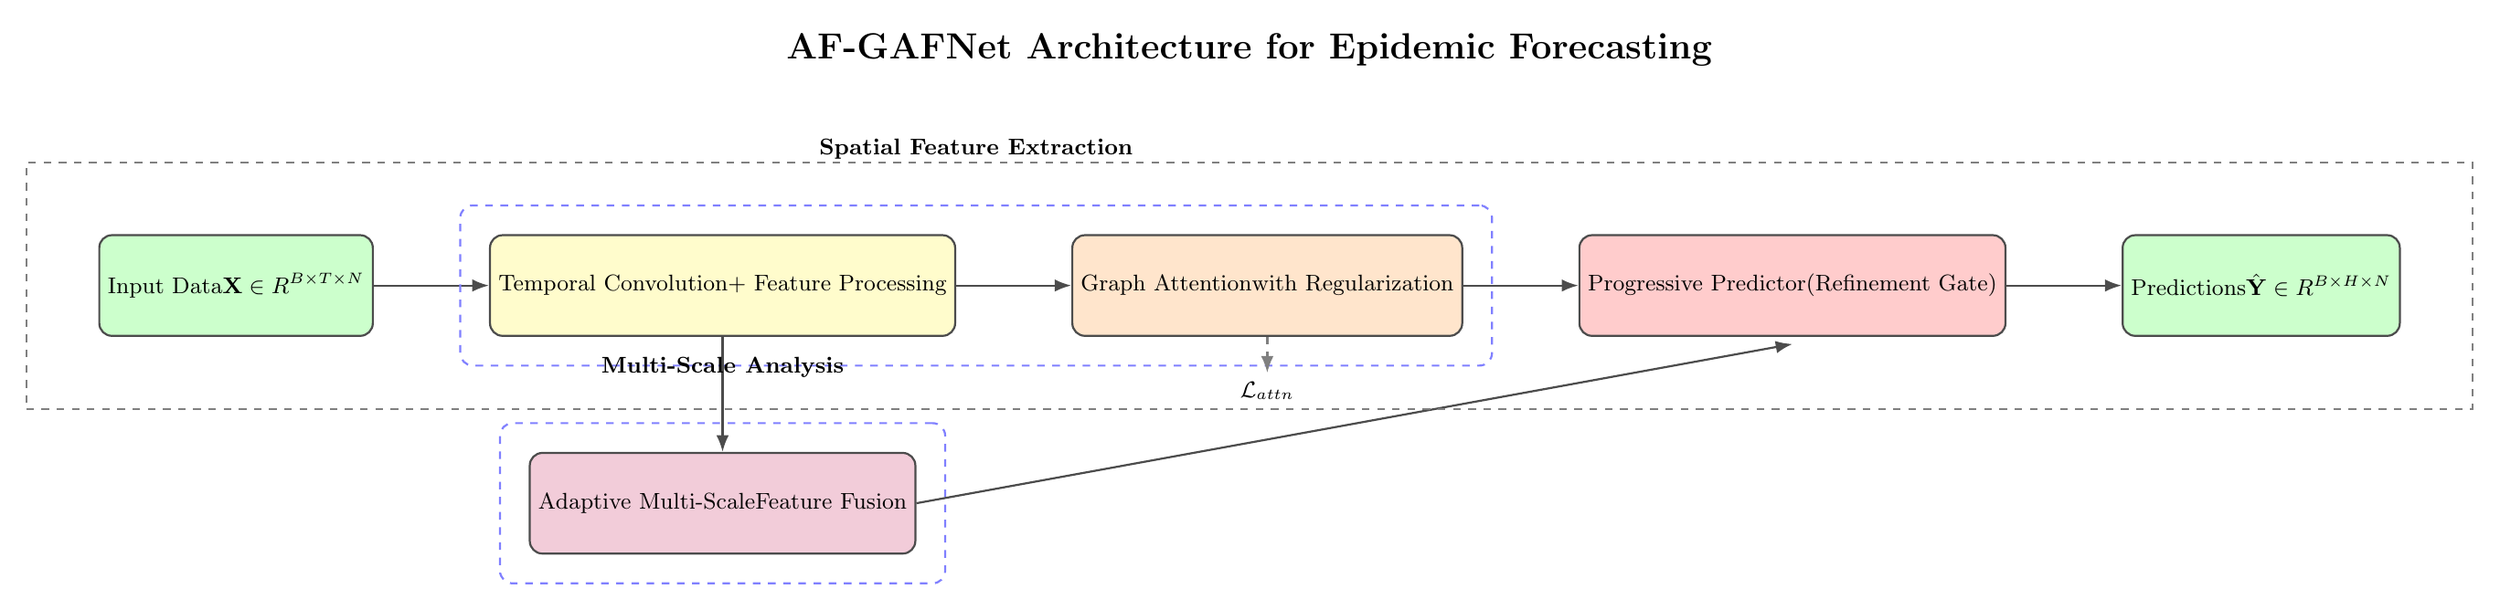
\begin{tikzpicture}[
    node distance=1.6cm and 1.6cm,
    every node/.style={font=\small},
    block/.style={
        draw=black!70, thick,
        minimum width=3.0cm, minimum height=1.4cm,
        rounded corners=5pt, fill=white
    },
    group/.style={
        draw=blue!50, thick, dashed,
        inner sep=0.4cm, rounded corners=5pt
    },
    arrow/.style={-Latex, thick, black!70},
    connector/.style={-Latex, thick, black!50, dashed}
]

% Input Layer
\node[block, fill=green!20] (input) {Input Data\\$\mathbf{X} \in \mathbb{R}^{B \times T \times N}$};

% Temporal Convolution + Feature Processing
\node[block, fill=yellow!20] (temp) [right=of input] {Temporal Convolution\\+ Feature Processing};
\draw[arrow] (input) -- (temp);

% Graph Attention Module
\node[block, fill=orange!20] (attn) [right=of temp] {Graph Attention\\with Regularization};
\draw[arrow] (temp) -- (attn);

% Group Feature Extraction Box
\node[group, fit={(temp) (attn)}] (featbox) {};
\node[above=0.5cm of featbox] {\textbf{Spatial Feature Extraction}};

% Adaptive Multi-Scale Feature Fusion Module (Feature Pyramid)
\node[block, fill=purple!20] (pyramid) [below=of temp] {Adaptive Multi-Scale\\Feature Fusion};
\draw[arrow] (temp.south) -- ++(0,-0.5) -| (pyramid.north);

% Group Multi-Scale Analysis Box
\node[group, fit={(pyramid)}] (pyramidbox) {};
\node[above=0.5cm of pyramidbox] {\textbf{Multi-Scale Analysis}};

% Progressive Predictor Module
\node[block, fill=red!20] (predictor) [right=of attn] {Progressive Predictor\\(Refinement Gate)};
\draw[arrow] (attn) -- (predictor);
% Straight arrow from pyramid to predictor, shifted to hit predictor.south
\draw[arrow] (pyramid.east) -- ($(predictor.south)+(0,-0.1)$);

% Output Layer
\node[block, fill=green!20] (output) [right=of predictor] {Predictions\\$\hat{\mathbf{Y}} \in \mathbb{R}^{B \times H \times N}$};
\draw[arrow] (predictor) -- (output);

% Auxiliary loss from Graph Attention (dashed arrow)
\node[below=0.5cm of attn] (aux) {\small $\mathcal{L}_{attn}$};
\draw[connector] (attn.south) -- (aux.north);

% Overall grouping box and title
\node[draw=black!50, thick, dashed, fit={(input) (output)}, inner sep=1cm] (overall) {};
\node[above=1.2cm of overall] {\Large \textbf{AF-GAFNet Architecture for Epidemic Forecasting}};
    
\end{tikzpicture}
\end{document}
